\documentclass{article}
\title{ECE 478-- Homework 3}
\usepackage{graphicx}
\usepackage{fancyhdr}
\usepackage{enumitem}
\usepackage{amsmath}
\usepackage{float}
\usepackage{amsmath}
\usepackage[margin=1in]{geometry}
\pagestyle{fancy}
\fancyhf{}
\fancyhead[L]{Gianni Avilan-Losee}
\fancyhead[C]{ECE 478}
\fancyhead[R]{Homework 3}
\fancyfoot[C]{\thepage}
\usepackage{microtype}
\usepackage{textcomp, gensymb}
\author{Gianni Avilan-Losee}
\setcounter{section}{2}
\begin{document}
\setcounter{section}{4}
\setcounter{subsection}{1}
\begin{enumerate}[label=\thesubsection]
	\item See Fig. 1 for the drawn diagram of the 2NOR gate under consideration. 
		\begin{figure}[H]
		  \centering
		  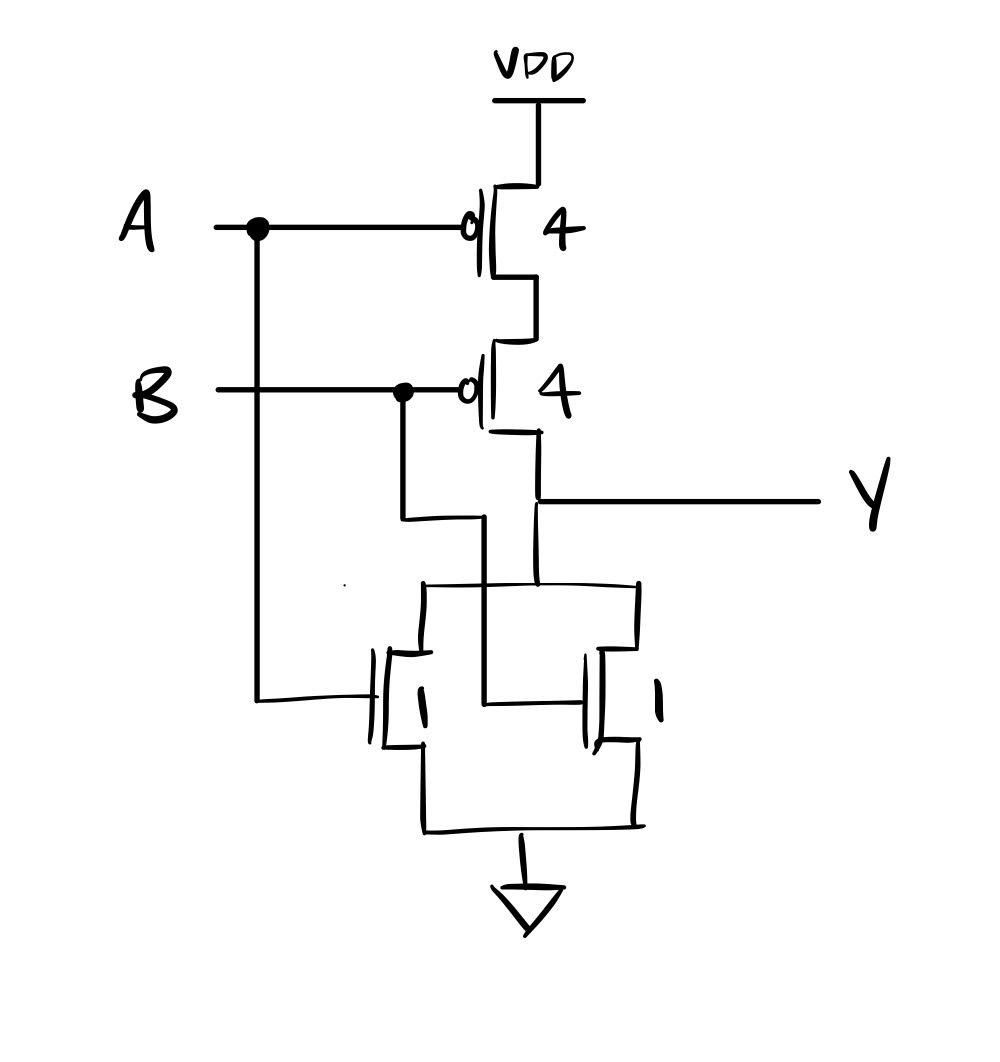
\includegraphics[width=0.4\textwidth]{homework-3_fig-1.jpg}
		  \caption{2NOR inverter with equivalent resistance to a unit inverter.}
		  \label{fig:2NOR}
		\end{figure}

		To derive the worst-case rising and falling delay as a function of \(h\) identical gates being driven by this one, we may first find the equivalent resistance and capacitance of each component by using the RC delay model, and then, using the Elmore delay model, we may estimate the effective delay as a function of \(h\) using the given RC values. 

		In the pull-up network, each pMOS transistor will show a gate and diffusion capacitance of \(4\mathrm{C}\) and an equivalent resistance of \(\frac{R}{2}\). In the pull-down network, each nMOS transistor will have a gate and diffusion capacitance of \(C\) and and an equivalent channel resistance of \(R\). 

		Beginning with worst-case falling delay \(t_{pdf}\), we consider worst-case resistance on the path between Y and GND to be the case when a single nMOS transistor is on, and its equivalent resistance is \(R\). Considering diffusion capacitances, the pMOS drain diffusion capacitance \(4\mathrm{C}\) is connected to Y, as well as two parallel nMOS drain diffusion capacitances \(C + C = 2C\). We may ignore any pMOS diffusion capacitances not on the path between Y and GND, as well as the two nMOS source diffusion capacitances, as these are shorted to GND through the substrate tap. In total, diffusion capacitance sums to \(4C + 2C = 6C\) for the driving 2NOR gate. On the other end, the gate capacitances of the pMOS and nMOS transistor at the load 2NOR gate sum to \(4C + C = 5C\), and increase with each added fanout gate. 

		Using the formula for Elmore delay, 
		\[
			t_{pdf} = \sum_{i}R_{is}C_{i} = R(6C+5hC) = (6C+5h)RC, 
		\]

		Worst-case rising delay \(t_{pdr}\) occurs when both pMOS series-connected pMOS transistors are on. In this case we have two nodes to deal with, as opposed to single node in the falling transition.  For the first node, at the junction between the source/drain of the series pMOS transistors, there is an equivalent resistance of \(\frac{R}{2}\) from this node to VDD, and a diffusion capacitance of \(4\mathrm{C}\), assuming a fully-contacted but shared diffusion node between the transistors.

		At the second node, corresponding to the output voltage, the equivalent resistance is comprised of both pMOS channels, so \(\frac{R}{2} + \frac{R}{2}\), and the total diffusion and gate capacitance at this node consists of \(6C + 5hC\), with \(h\) once again representing the number of load 2NOR gates. Summing the resistance and capacitance at the two nodes using the Elmore delay formula,

		\[
			t_{pdr} = \sum_{i} R_{is}C_i = \frac{R}{2}(4C) + R(6C+5hC) = (8+5h)RC.
		\]
	\setcounter{subsection}{2}
	\item The following (Fig. 2) is the stick diagram for a 2NOR gate, optimized to reduce delay due to parasitic capacitances: 
		\begin{figure}[H]
		  \centering
			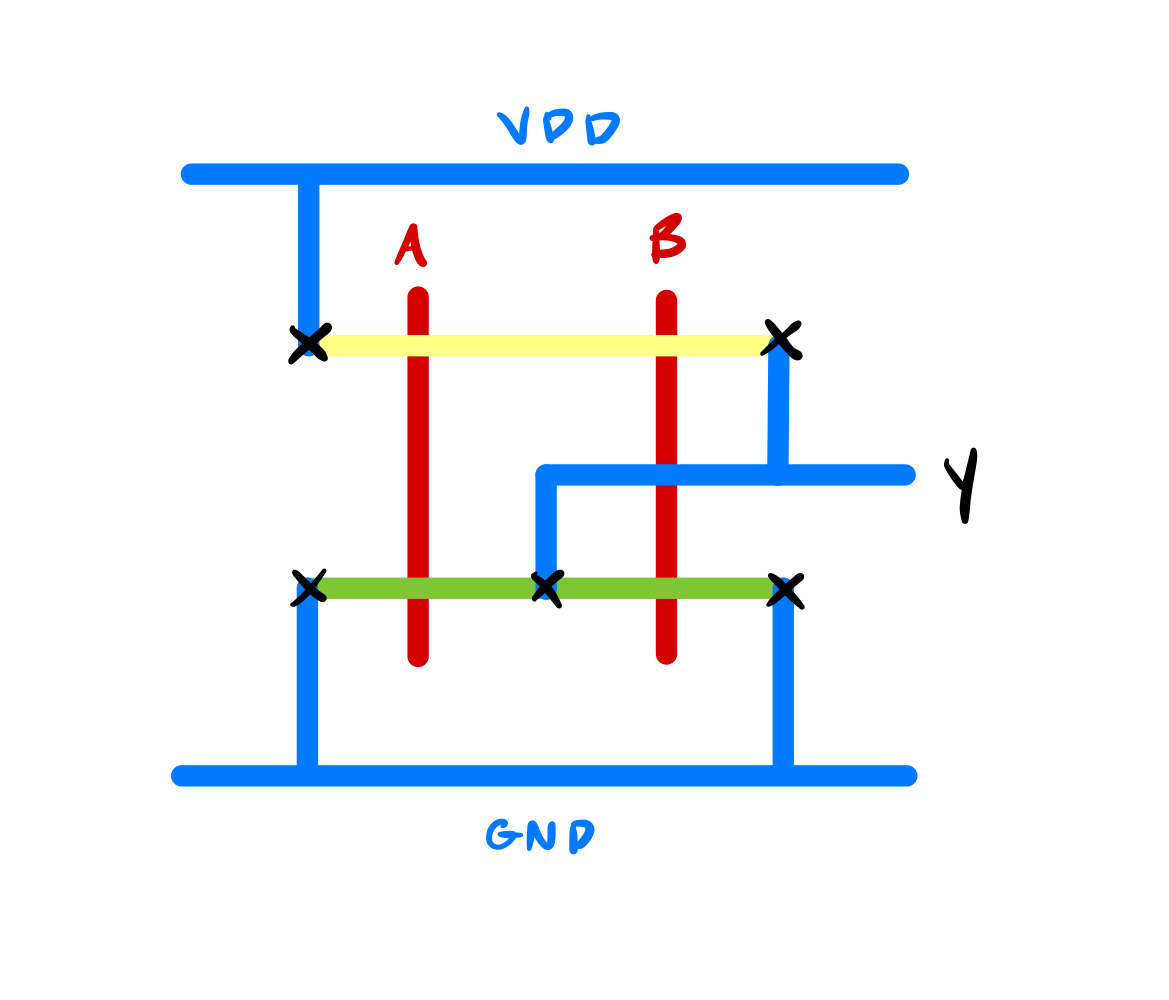
\includegraphics[width=0.6\textwidth]{homework-3_fig-2.jpg}
		  \caption{2NOR stick diagram}
		  \label{fig:2NOR stick}
		\end{figure}
		Starting with rising delay, we assume that the shared diffusion node between the series pMOS inverters is not contacted and that the contacted diffusion node at the drains of the two parallel nMOS transistors is shared, we estimate a diffusion capacitance of \(2\mathrm{C}\) at node 1 and a total gate/diffusion capacitance of \(5C + 5hC\) at the output node, with no change in equivalent resistance, \[
			t_{pdr} = \frac{R}{2}(2C) + R(5C + 5hC) = RC(6 + 5h).
		\] 
		For falling delay, we again assume a shared, contacted diffusion between the two parallel nMOS drains, so 
		\[
			t_{pdf} = R(5C+5hC) = RC(5+5h).
		\]
		\setcounter{subsection}{3}
	\item For an AOI21 gate, with unit inverter-equivalent rising and falling resistances, Fig. 3 shows the circuit diagram (with transistor sizing), stick diagram optimized to reduce delay, and worst-case rising and falling RC equivalent circuits, estimating lower diffusion capacitances at shared, fully contacted nodes and shared, uncontacted nodes.
		\begin{figure}[H]
		  \centering
		  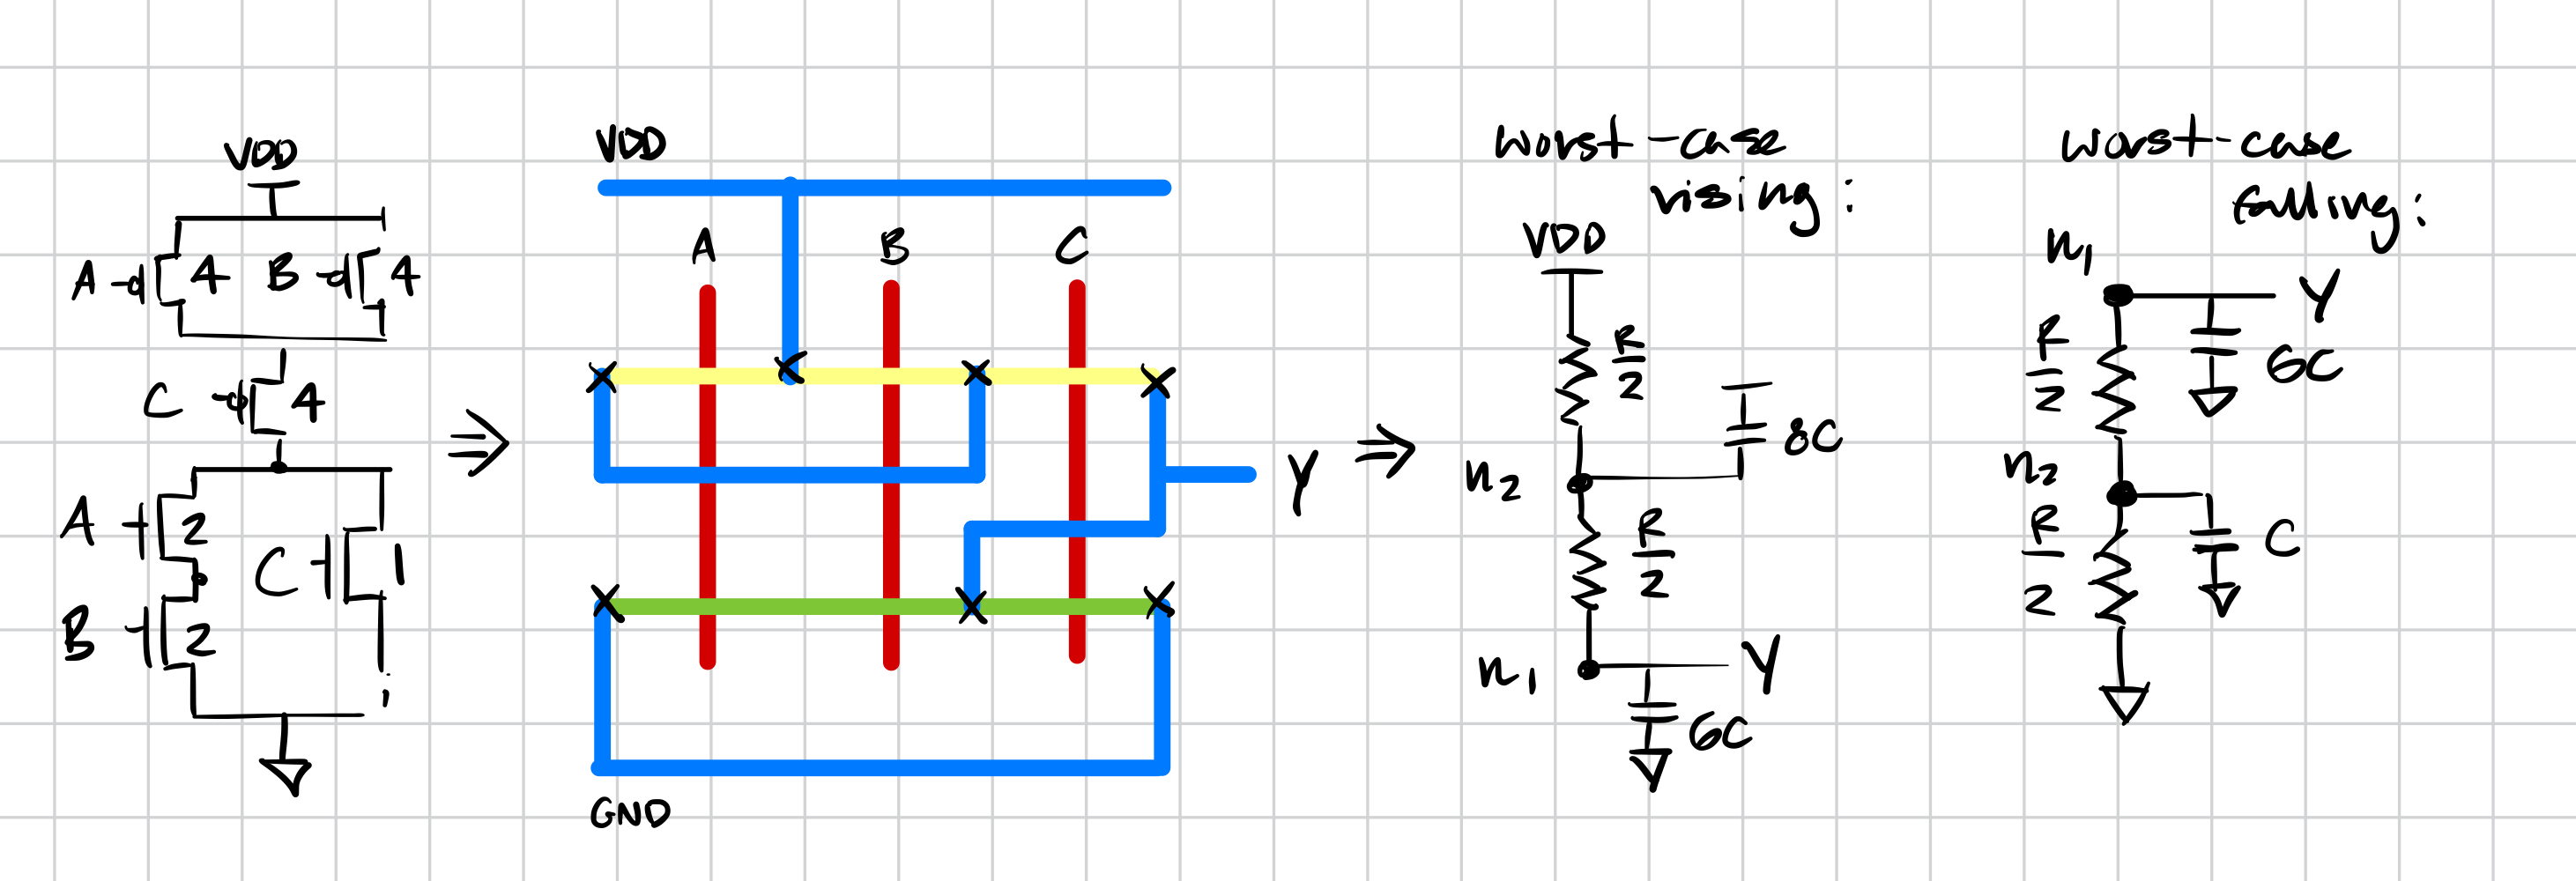
\includegraphics[width=0.8\textwidth]{homework-3_fig-3.jpg}
		  \caption{AOI21 schematic, stick diagram, and RC equivalent circuits}
		  \label{fig:AOI21}
		\end{figure}
		Using the Elmore delay model to estimate rising and falling delay, respectively, 
		\begin{align*}
		 &\tau_{pdr} = R(6C) + \frac{R}{2}(8C) = 10RC \\
		 &\tau_{pdf} = R(6C) + \frac{R}{2}(C) = \frac{13}{2}RC = 6.5RC.
		\end{align*}
		\setcounter{subsection}{5}
	\item Fig. 4 shows a comparison between normalized delay \(d\) as a function of fanout \(h\) for a 2NOR and 2NAND gate, accounting for parasitic delay \(p\). A comparison shows that 2NOR and 2NAND gates share equal parasitic delays, and thus share an equal normalized delay \(d\) when not driving other gates. However, when connected as the drivers to \(h\) fanout gates, 2NAND gates perform better as more fanout gates are added, where the difference in delay between the two grows larger with each added load gate.
			\begin{figure}[H]
			  \centering
			  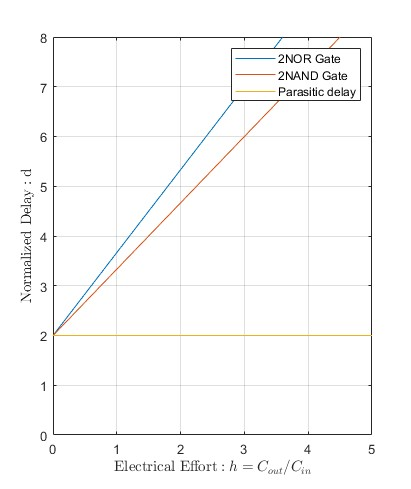
\includegraphics[width=0.5\textwidth]{homework-3_fig-4.jpg}
			  \caption{Logical effort comparison between 2NOR and 2NAND gates}
			  \label{fig:logical}
			\end{figure}
			\setcounter{subsection}{9}
		\item Fig. 5 shows the circuit diagram for a 4NAND gate with transistor sizing chosen for unit inverter-equivalent resistances. 
			\begin{figure}[H]
			  \centering
			  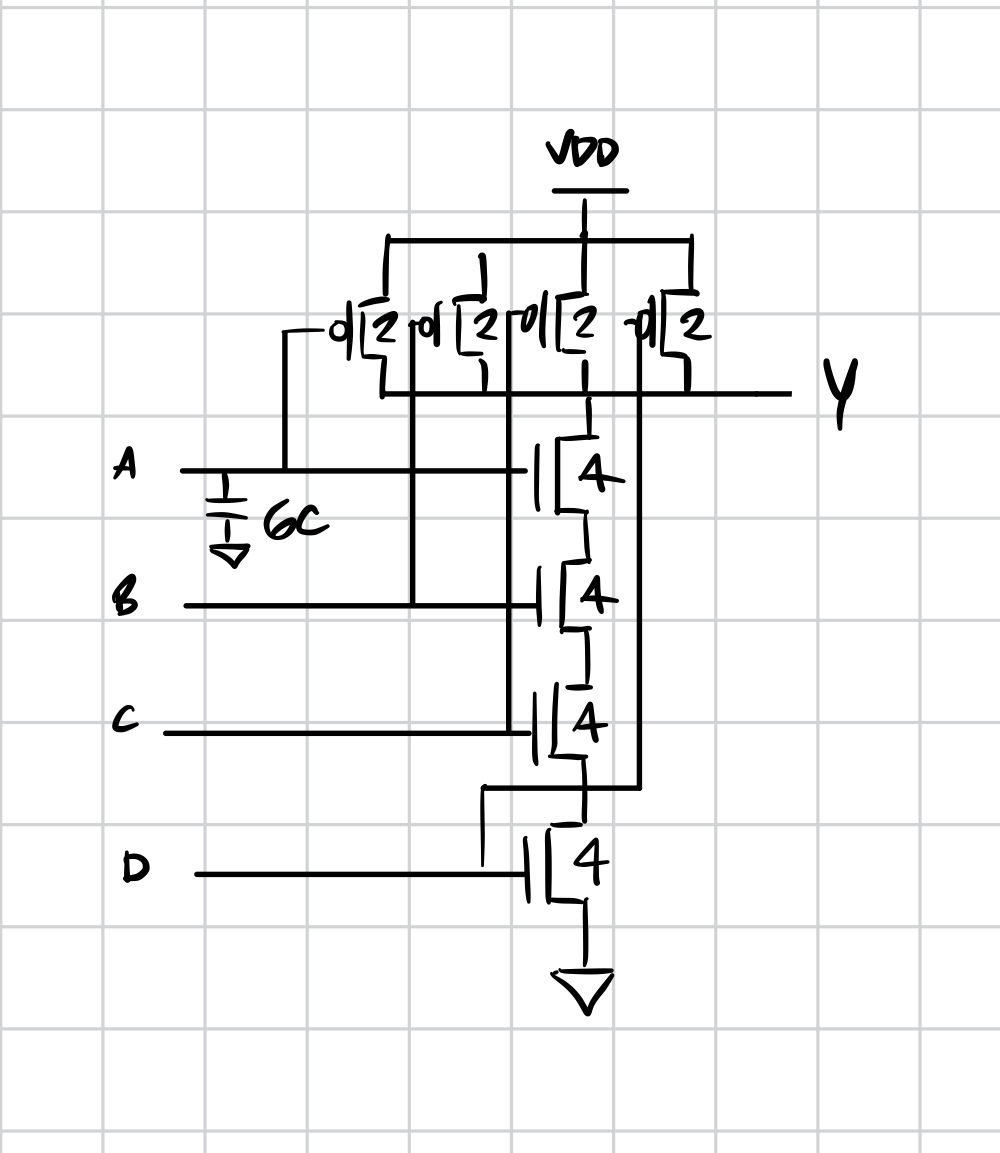
\includegraphics[width=0.5\textwidth]{homework-3_fig-5.jpg}
			  \caption{4NAND gate with unit inverter-equivalent transistor widths}
			  \label{fig:label}
			\end{figure}
			At each input, we estimate gate capacitance to be the sum of nMOS and pMOS gate capacitances, and so the input capacitance \(C_{in} = 6C\). For a unit inverter, \(C_{in} = 3\), and so logical effort, the ratio between this gate's input capacitance and an equivalent unit inverter's input capacitance, is \(g = \frac{6}{3}\).
			setcounter{subsection}{19}
		\item The input capacitance of the given unit inverter is \(C_{\mathrm{in}}=4C\). Therefore, the logical effort of a 2NAND fabricated using the same process, where \(R_{\mathrm{pMOS}} = 3R_{\mathrm{nMOS}}\), is the sum of the gate capacitance of the two driven input gates, \(C_{\mathrm{in}} = 2C+3C = 5C\), and so logical effort \(g_{\mathrm{2NAND}}=\frac{5}{4}\). For a 2NOR gate fabricated using the same process, \(C_{\mathrm{in}} = C + 6C = 7C\), and so logical effort \(g_{\mathrm{2NOR}} = \frac{7}{4}\).
\end{enumerate}
\end{document}
